\chapter{Analisi e testing del sistema}
Le reti che il sistema intende monitorare sono potenzialmente estese e diversificate, sia come natura di dispositivi che come protocolli infrastrutturali. È infatti ragionevole pensare che una rete di home automation impieghi protocolli come Ethernet e 802.15.4 su IPv4, o che un network di sensori per smart cities impieghi tecnologie Sub-1GHz su IPv6. È importante quindi che il sistema di monitoraggio sia flessibile e sia in grado di poter operare con tutte, o buona parte, di queste tecnologie. Potenzialmente l'utente potrebbe registrare decine, centinaia e addirittura migliaia di azioni ed è quindi altrettanto importante che il sistema risponda correttamente alla richiesta di aumento di azioni.
\\In questo capitolo svilupperemo un'analisi del sistema di monitoraggio in merito ai requisiti esposti all'inizio di questo scritto e cercheremo di capire se effettivamente siano stati o meno rispettati.
\\Si cercherà inoltre di dare una fotografia sulle possibili applicazioni d'uso e sugli scenari possibili, oltre che di dare uno sguardo al futuro e alle possibili implementazioni che possono rendere il sistema migliore e quali siano le aree di intervento coinvolte.

\section{Scalabilità, portabilità e interoperabilità}
Innanzitutto è utile capire se il sistema sviluppato scala correttamente al crescere delle azioni registrate: se così non fosse non potrebbe essere certamente impiegato in scenari di tipo IoT, dove i dispositivi da monitorare sono potenzialmente migliaia e dove potenzialmente più utenti potrebbero voler monitorare la stessa risorsa.
\\Si è cercato quindi di stimare quale fosse il memory footprint dell'applicazione server, valutando la crescita di utilizzo in base all'aumentare dei thread gestiti. Le stime sono state effettuata direttamente dall'interno del {\tt CoapAgent} utilizzando la formula seguente:
\lstset{title=Calcolo della memoria in utilizzo dalla JVM}
\begin{lstlisting}
Runtime.getRuntime().totalMemory() - Runtime.getRuntime().freeMemory()
\end{lstlisting}
\vspace{0.50cm}
La stima ottenuta mediante la classe {\tt Runtime} non è ovviamente precisa al byte, in quanto risente anche della memoria utilizzata dalla stessa Java Virtual Machine per gestire l'applicazione, ma può comunque dare un'idea di quella che potrebbe essere la necessità di memoria del sistema in questione.
\\Dalle stime effettuate sono stati ottenuti i seguenti risultati:
\begin{table}[h]
\centering
\caption{Utilizzo di memoria in base al numero di thread crescente. Le unità sono espresse in KB.}
\vspace{0.5cm}
\label{my-label}
\begin{tabular}{|l||c|c|c|c|c|c|}
\hline
 & 1 & 10 & 20 & 50 & 100 & 200 \\
\hline
\emph{Observe} & 126 & 1292 & 2445 & 6240 & 12876 & 26157 \\
\hline
\emph{Periodic} & 108 & 1240 & 2318 & 6073 & 12322 & 25041 \\
\hline
\end{tabular}
\end{table}
\\Il memory footprint della sola istanza server è invece intorno ai 23,5 MB.

\begin{figure}[p]
\centering
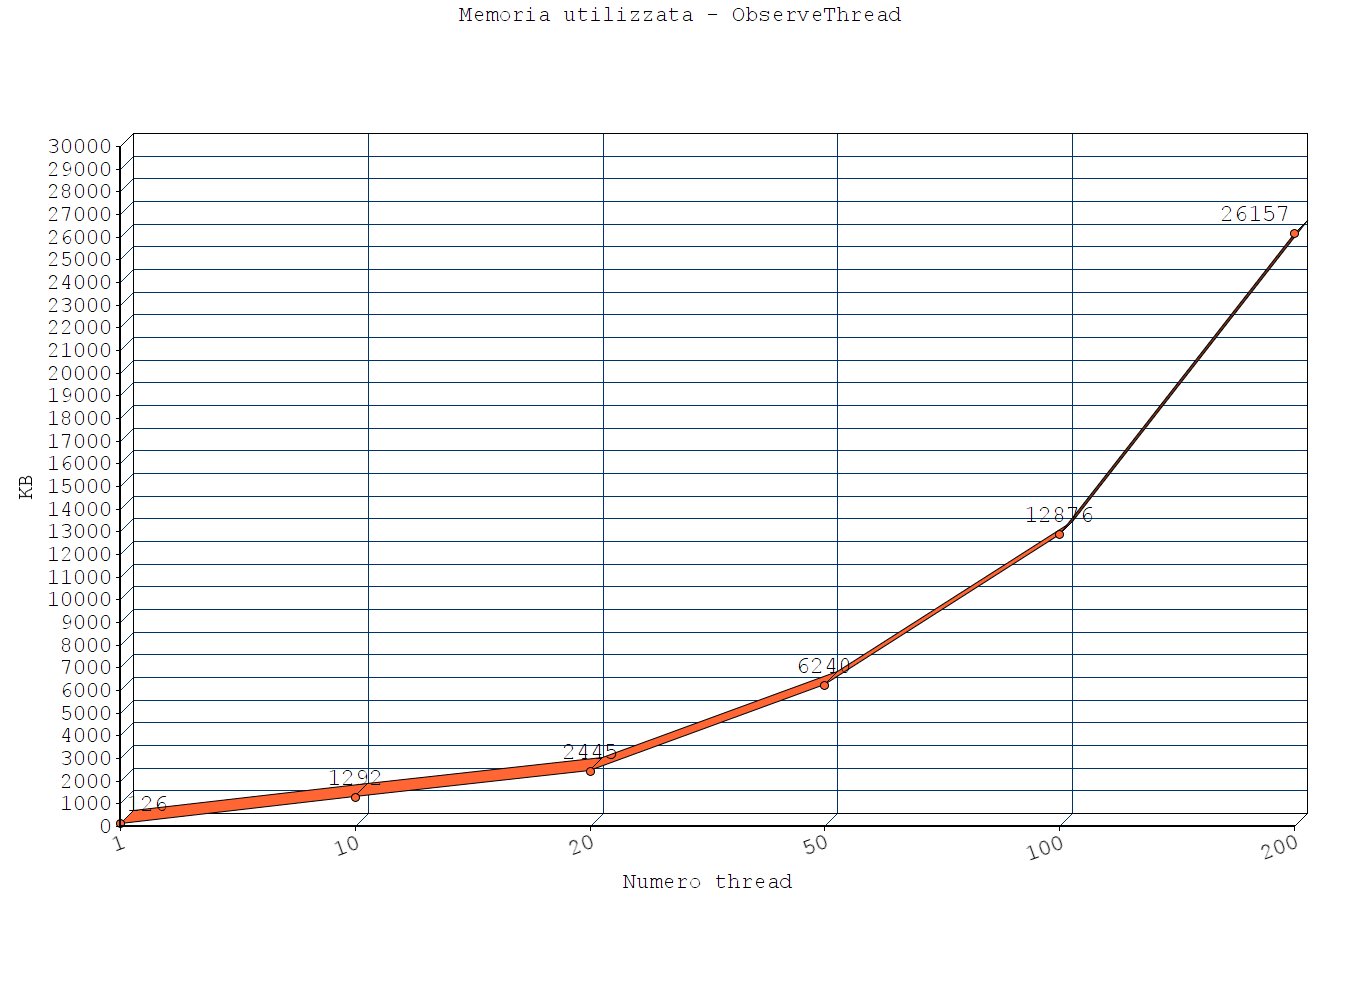
\includegraphics[width=\textwidth]{immagini/observe.png}
\caption{\textit{La crescita di memoria per i thread {\tt Observe}}}
\end{figure}
\begin{figure}[p]
\centering
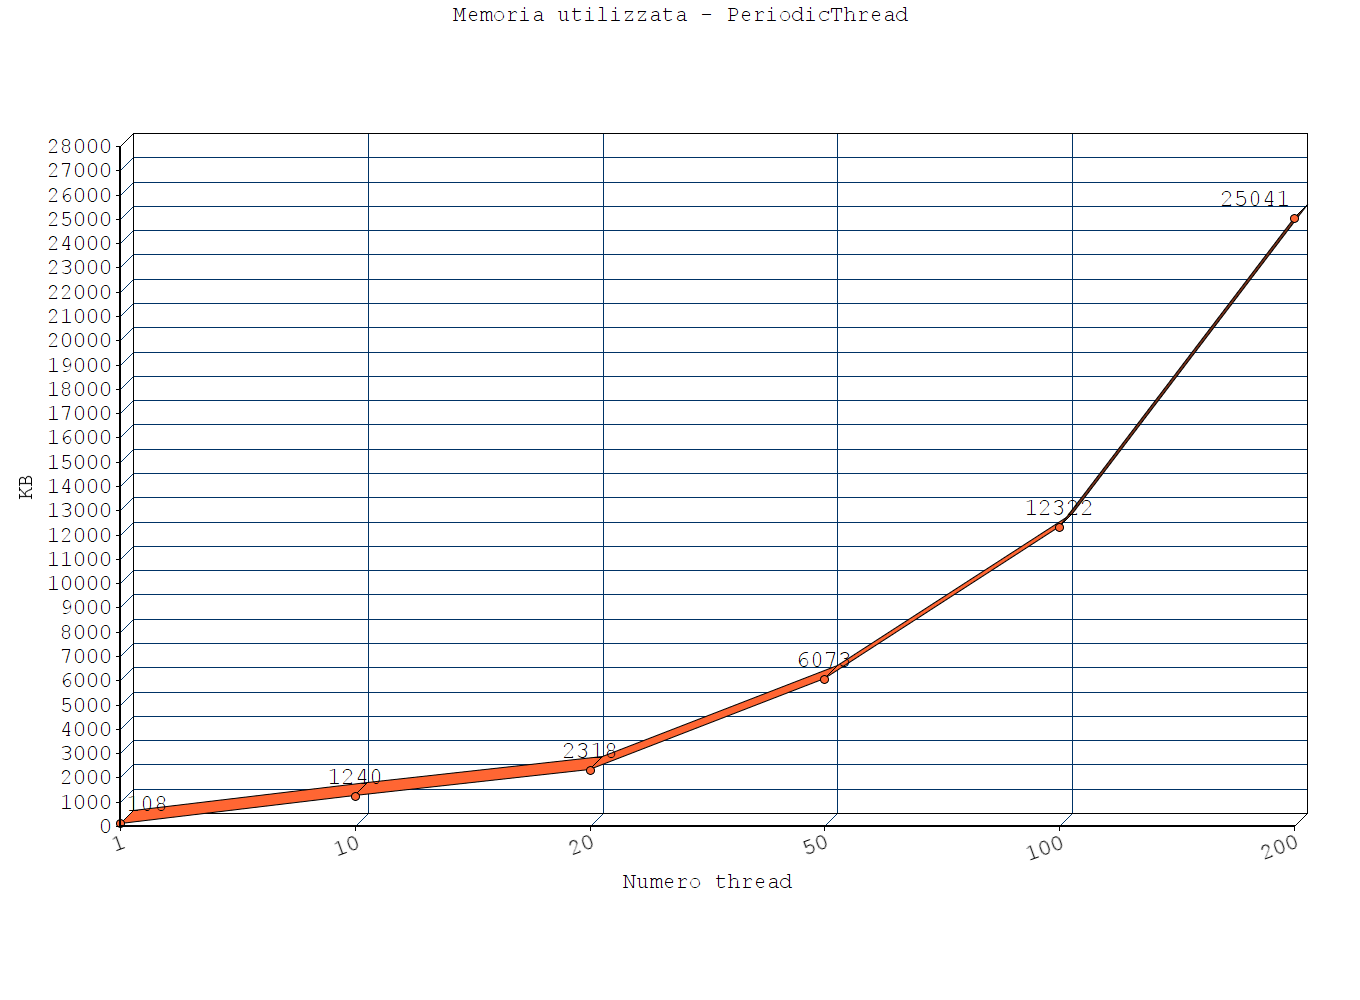
\includegraphics[width=\textwidth]{immagini/periodic.png}
\caption{\textit{La crescita di memoria per i thread {\tt Periodic}}}
\end{figure}

\vspace{1.0cm}
Come è possibile notare la crescita di richiesta di memoria è abbastanza lineare, permettendo al sistema di essere sufficientemente scalabile e relativamente leggero. La leggerezza del sistema potrebbe permettere di installare il sistema di monitoraggio su qualunque dispositivo che sia in grado di sostenere la Java Virtual Machine, come per esempio il noto Raspberry Pi, garantendo la possibilità di utilizzo non solo su sistemi distribuiti ad alte prestazioni ma anche in ambienti più ristretti come un'abitazione o una piccola azienda.
\\\\È stata testata la portabilità del sistema su sistemi operativi differenti (Windows e Linux) con successo, riscontrando una differenza prestazionale quasi nulla tra i due sistemi. La portabilità è un fattore importante in quanto il sistema server potrebbe essere potenzialmente configurato e installato su sistemi e architetture differenti per rispondere ad esigenze d'uso differenti.
\\Il sistema di monitoraggio è predisposto per poter funzionare con interfacce differenti da quella Web utilizzata, essendo necessario semplicemente effettuare delle chiamate RPC alla cloud, e può quindi essere attivato, per esempio da una applicazione per smartphone oppure in automatico da un altro server.
\\\\Il sistema è anche interoperabile, in quanto è in grado di monitorare una qualunque risorsa che sia in grado di comunicare tramite protocollo CoAP che, essendo estremamente leggero e versatile, è adatto a funzionare sulla stragrande maggioranza degli smart objects. È stata inoltre testata la possibilità di monitorare sia reti basate su protocollo IPv4 che IPv6 che misto, con grande successo, garantendo al sistema di essere in grado di prelevare dati da reti di diversa natura.

\section{Scenari d'uso}
I possibili scenari d'utilizzo del sistema di monitoraggio sono molteplici: si potrebbe immaginare, per esempio, un sistema distribuito sul quale la cloud è installata su di un server o magari un cluster in cloud, il DBMS è installato su di un altro server e l'interfaccia Web su un terzo server. Le reti da monitorare potrebbero essere, per esempio, reti di sensori che rilevano l'occupazione dei parcheggi pubblici in una città e l'utente, tramite interfaccia Web o tramite app per smartphone, potrebbe monitorare i parcheggi sotto casa per sapere in tempo reale quando uno diventa libero, utilizzando un connettore che lo avvisa via email.
\\Oppure cloud, DBMS e interfaccia potrebbero essere installati su di un PC in casa che monitora lo stato di alcuni sensori, come sensori di temperatura e umidità, sensori di movimento, di rilevamento gas ecc... per aggiornare un profilo Twitter pubblico e mantenere lo storico delle temperature nelle varie stanze ed essere allertati quando viene rilevata una fuga di gas.
\\\\O ancora, il sistema cloud potrebbe essere di dominio pubblico e un'azienda potrebbe creare la propria interfaccia per monitorare lo stato di alcuni sensori posti all'interno dell'azienda stessa, per avere una stima della produzione giornaliera, per esempio, o per stimare l'utilizzo di corrente. I dati potrebbero essere inviati tramite un connettore customizzato ad un database interno all'azienda per essere successivamente analizzati e perfezionare così l'andamento dei processi aziendali.
\\\\Le possibilità offerte sono tantissime e gli scenari profilabili altrettanti. È necessario solamente avere a disposizione una rete di sensori che siano in grado di comunicare tramite protocollo CoAP.

\section{Possibili sviluppi futuri}
Alcuni possibili sviluppi futuri potrebbero rendere il sistema cloud ancora più interessante. Delle possibili espansioni potrebbero essere:
\begin{itemize}
\item L'aggiunta di nuovi connettori, oltre al già presente Twitter, come Facebook, Telegram, email, pubblicazione di pagine HTML ecc...
\item La possibilità per la cloud di effettuare automaticamente la discovery di nuove risorse nella rete e notificare la presenza all'utente tramite connettori oppure creare automaticamente un'azione di monitoraggio per le nuove risorse.
\item La creazione di una vera e propria API per l'accesso alla cloud, costruendo uno strato di astrazione per le chiamate XML-RPC, rendendo così disponibili le operazioni di creazione e cancellazione di azioni anche da interfacce esterne senza necessariamente effettuare chiamate RPC.
\item L'aggiunta di nuove chiamate RPC alla cloud, con la possibilità di ottenere il livello di carico del sistema in tempo reale. Sarebbe possibile effettuare questa espansione sfruttando lo stesso paradigma di monitoraggio, rendendo la cloud stessa una risorsa, uno smart object che notifica in tempo reale a sè stesso, e quindi all'utente che ne ha richiesto il monitoraggio, il proprio stato.
\item L'inclusione di altri protocolli IoT, come MQTT, per rendere possibile il monitoraggio sul maggior numero possibile di smart objects e ampliare ulteriormente l'area di operabilità del sistema.
\end{itemize}
